\section{Architektur \textnormal{\textsf{\small{Markus Böbel}}}}

Durch das Echtzeit-Spielkonzept des Planspiels ist es für die Anwendung von Nöten ständig Daten, auszuwerten und zu berechnen. Damit diese Berechnungen erfolgreich durchgeführt werden können, müssen diese unabhängig von der Präsenz der Spieler durchgeführt werden. Dies wird erreicht durch die Einrichtung eines einfachen verteilten Systems, indem die Programmlogik auf einem abgeschlossenen Server liegt, während sich die Spieler lediglich nötige Information anfragen oder ihr Handeln dem Server mitteilt.
Wenn nun ein Spieler das Spiel für eine gewisse Zeit unterbricht, können andere Spieler in dieser Zeit das Spiel fortführen.

Als der Software Architektur liegt ein eine einfache Three-Tier-Architektur. (siehe Abbildung \ref{abb:architektur})
Wie der Name es vermuten lässt, besteht eine solche Architektur aus drei grundlegenden Elementen.

\begin{description}
	\item[Datenschicht] Die Datenschicht dient der Datenpersistenz und besteht meist aus einer Datenbank.
	\item[Logikschicht] Diese Schicht bearbeitet die Daten der Datenschicht und bringt diese in einen semantischen Zusammenhang. 
	\item[Präsentationsschicht] Bei dieser Schicht werden die hergerichteten Daten der Logikschicht präsentiert. Sie stellt sozusagen die Schnittstelle zum späteren Spieler da, weil dieser bloß auf der Präsentationsschicht handelt.
\end{description}
Der Grund für diese Schichtentrennung ist die einfachere Austauschbarkeit der verschiedenen Bestandteile. Wenn zum Beispiel das Datenbanksystem erneuert werden soll, so ist dies ohne großen Aufwand möglich. Das Gleiche gilt auch für die anderen Bestandteile.

Im konkreten Falle des Planspiels besteht die Präsentationsschicht aus einer Webseite. Diese sendet die Eingaben des Benutzers weiter an eine REST-Schnittstelle (siehe Kapital \ref{sec:rest}). Diese wird auf einem Tomcat Server initialisiert, auf welchem die Anfragen bearbeitet und das Spielkonzept umgesetzt werden.


\begin{figure}[h]
	\centering	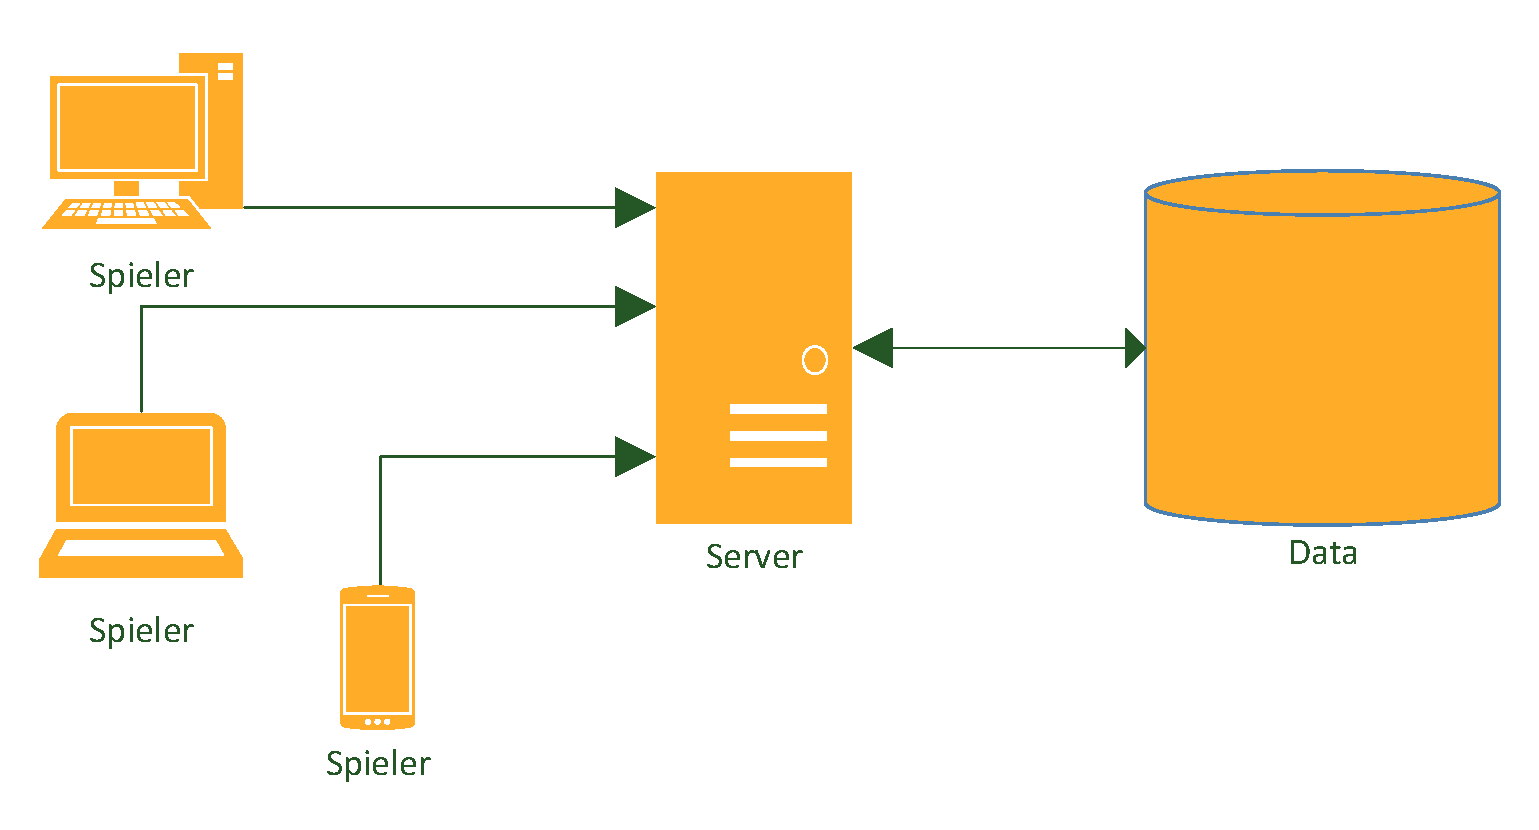
\includegraphics[width=\textwidth]{img/architektur}
	\captionsetup{format=hang}
	\caption{
		\label{abb:architektur}Aufbau der Applikationsarchitektur}
\end{figure}

 Auf die Datenschicht wird im Falle des Planspiels verzichtet, da es keine Voraussetzung die Daten persistent zu halten und dies einen hohen Mehraufwand darstellen würde. Daraus folgt, dass die Daten nun zur Laufzeit bearbeitet und verwaltet werden.
 Im Falle eines Serverneustartes oder -ausfalls würden folglich alle Planspieldaten wie zum Beispiel Spielstände verloren gehen. Da aufgrund von Wartungsarbeiten Serverneustarts nichts Ungewöhnliches ist und es sich bei dem Planspiel um ein langwieriges Spiel handelt, ist es von Nöten eine Datenschicht nachträglich zu implementieren. 
